\documentclass[a4paper]{article}

%% Language and font encodings
\usepackage[english]{babel}
\usepackage[utf8x]{inputenc}
\usepackage[T1]{fontenc}

%% Sets page size and margins
\usepackage[a4paper,top=3cm,bottom=3cm,left=3cm,right=3cm,marginparwidth=1.75cm]{geometry}

%% Useful packages
\usepackage{amsmath}
\usepackage{subcaption}
\usepackage{graphicx}
\usepackage{media9}
\usepackage[colorinlistoftodos]{todonotes}
\usepackage[colorlinks=true, allcolors=blue]{hyperref}
\usepackage{setspace}
\usepackage{tikz}
\usepackage{hyperref}
\def\repository{https://github.com/ahoereth/pysnake}
\def\repositoryurl#1{\repository/blob/master/#1}
\def\coderef#1{\href{\repositoryurl{#1}}{\texttt{#1}\footnote{\url{\repositoryurl{#1}}}}}
\def\lineref#1#2{\coderef{#1\#L#2}}
\def\layersep{2.5cm}

\title{PySnake -- Playing Snake with ANNs\\\normalsize{Final Project for ``Implementing Artificial Neural Networks with TensorFlow''}}
\author{Sebastian Höffner, Alexander Höreth, Ann-Christin Meisener, Andrea Suckro}

\begin{document}
\onehalfspacing
\maketitle

\begin{abstract}
As our final project we implement two different artificial neural network approaches with TensorFlow to explore their capability of playing Snake. In this report we will report our implementations and parameters as well as our results. Additionally we will evaluate the artificial neural networks considering their performance against each other and against human players and draw the conclusion that the neural network approaches, while promising,  perform less than optimal for this problem.
\end{abstract}


%%%%%%%%%%%%%%%%%%%%%%%%%%%%%%%%%%%%%%%%%%%%%%%%%%%%%%%%%%%%%%%%%%%%%%
%%%%%%%%%%%%%%%%%%%%%%%%%%%%%%%%%%%%%%%%%%%%%%%%%%%%%%%%%%%%%%%%%%%%%% 
\section{Introduction}
Humans are very good at playing games. They are not only very good, they excel at many different kinds of games, and they play them for pleasure because it comes in so natural -- in fact, children seem to learn through
play\cite{wiki:ltp}. However, for computers, ``playing'' is a difficult task. While some breakthroughs have been achieved with classical rule based and optimization focused strategies in the past (cf. Deep Blue\cite{CAMPBELL200257} and Watson\cite{FERRUCCI201393}), more recent game playing strategies involve heavy use of artificial neural networks (ANNs). One of the most notable instances is DeepMind, which uses Q-learning to learn to play several Atari games\cite{mnih2013}. What is novel about this approach is that it is implemented completely game agnostic, it only gets the current game state as its input and produces an action as output.

Inspired by DeepMind's success, we decided to teach our computers to play
Snake. In it, the player controls a snake that can be moved over the game board to collect food tokens. Every time the snake collects a food token, it grows by one in size and a new food token is spawned on a random background location. The game is lost when the snake collides with itself, which becomes increasingly hard as the snake grows with each food token, and is won when the game board is completely
covered by the Snake. 

Our goal is to write an ANN using the framework TensorFlow\cite{tensorflow2015} which, in the best case, outperforms human players. We explore two different approaches, Q-learning and an evolutionary algorithm, and compare these to human performances and a systematic automatic solver. To compare them, we will evaluate scores and as a secondary metric the number of executed steps before a game is lost. 

In this report we describe in detail which components are implemented to
complete the final project. All code can be found on
GitHub\footnote{\url{\repository}} and exclusively
uses Python 3.6\footnote{\url{https://python.org}} to solve the tasks. The project is split into several small parts: the game implementation, its visualization, and different snake player implementations. The report starts by giving an overview over these individual parts. Then the important topics, the evolutionary algorithm as well as the Q-learning approach, will be explained and explored in depth, followed by a performance
evaluation of both. In the discussion the report concludes with some final remarks about the challenges that were faced and the results. Results can be found by following the links in section~\ref{sec:res} of this report.


%%%%%%%%%%%%%%%%%%%%%%%%%%%%%%%%%%%%%%%%%%%%%%%%%%%%%%%%%%%%%%%%%%%%%%
%%%%%%%%%%%%%%%%%%%%%%%%%%%%%%%%%%%%%%%%%%%%%%%%%%%%%%%%%%%%%%%%%%%%%%
\section{The Snake game}
For the project we build our own basic implementation of the Snake game (see Figure~\ref{fig:sboard}). It is a game in which a player controls an avatar which is composed of a chain of several segments, depicting a snake. The game takes place in a two dimensional environment, in which the snake can move along an implicit grid. Each segment occupies one of the grid cells. One segment is considered the snake's head and players can control where it shall move by supplying one direction: up, down, left, or right. The snake then moves by occupying the next cell adjacent to the snake's head in the direction the player provides and the last cell becomes unoccupied. In many popular game versions the snake advances automatically every few milliseconds, however for simplicity, in our game the snake only advances one step per command.

\begin{figure}
  \centering
  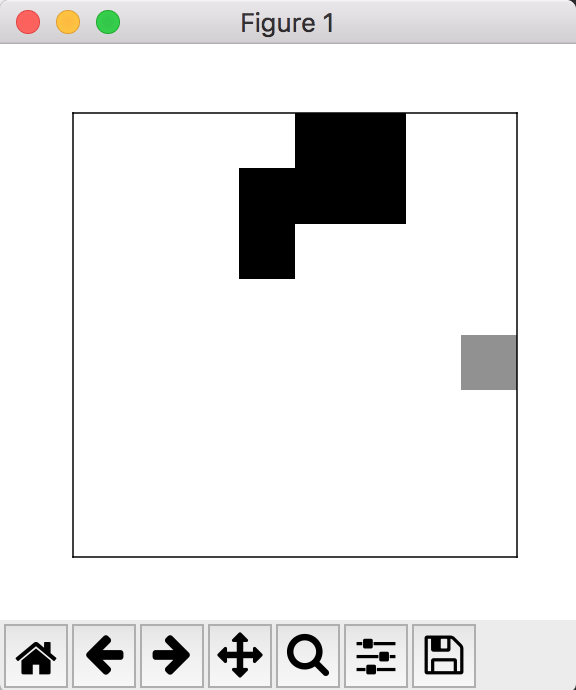
\includegraphics[width=.5\textwidth]{SnakeBoard.png}
  \caption{\label{fig:sboard}The graphical user interface of the Snake game. To control the snake, several different controllers exist: the human controller allows to use the arrow keys to move around, while other controllers are not dependent on the visualization}
\end{figure}

The goal in Snake is to feed the snake with food, which randomly appears inside the grid. There is always one food token inside the grid, and once the snake reaches the cell occupied by that token, it consumes it and a new food spawns at some other random location. However, when the snake eats one food, its length increases by one, resulting in a longer tail. Eventually the game is lost: either by hitting a wall, or by hitting another snake segment with the snake's head.

For experimental reasons we implement multiple variations of the game. In the original game the snake looks all the same and a player can only determine which part is the head and which the tail by considering a history of moves. To simplify this detection one can instantiate the snake class such that the snake head is highlighted by another gray shade -- a distinction which might or might not help some of our networks to train better. Additionally we allow players to toggle walls. If walls are enabled, the game is lost when the snake's head would move out of the border, but if they are disabled, the snake will just reappear on the opposite side of the board.

The graphical user interface (GUI) is realized with a matplotlib\cite{Hunter:2007} animation. It can be plugged in as needed, and is in general disabled while we train our ANNs. We use it to check our results and for the human player -- additionally the systematic snake (see below) is visualized with this interface.


%%%%%%%%%%%%%%%%%%%%%%%%%%%%%%%%%%%%%%%%%%%%%%%%%%%%%%%%%%%%%%%%%%%%%%
%%%%%%%%%%%%%%%%%%%%%%%%%%%%%%%%%%%%%%%%%%%%%%%%%%%%%%%%%%%%%%%%%%%%%%
\section{The different Players -- Design and Architecture}


%%%%%%%%%%%%%%%%%%%%%%%%%%%%%%%%%%%%%%%%%%%%%%%%%%%%%%%%%%%%%%%%%%%%%%
%%%%%%%%%%%%%%%%%%%%%%%%%%%%%%%%%%%%%%%%%%%%%%%%%%%%%%%%%%%%%%%%%%%%%%
\subsection{Human Snake}
This player is not providing any logic to control the snake, but allows for a human player to play the game. We use this player to collect our data for the human level performance base rate. It is also a helpful addition to test the game code and the GUI. The snake is controlled with the arrow keys and each new position of the snake is updated in the visualization \ref{fig:sboard}. The game is terminated when it is lost or won and has to be restarted if one wishes to play another round.


\subsection{Systematic Snake}
The systematic approach solves the game for even-sized boards (that is, both sides have an even size). It uses a simple Hamilton cycle (see Figure~\ref{fig:hamiltoncycle} and just repeatedly moves across the whole board to survive as long as possible and eventually gather all food. Thus the results for the systematic snake tend towards lots of steps with the maximum score.

\begin{figure}
	\centering
    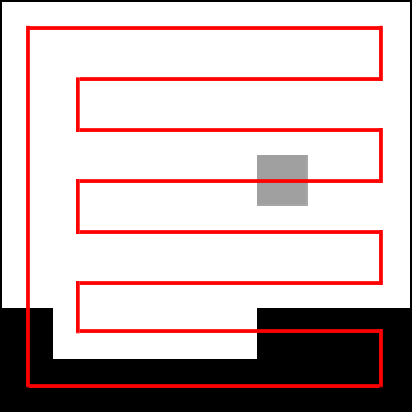
\includegraphics[width=.5\textwidth]{hamiltoncycle.jpg}
    \caption{\label{fig:hamiltoncycle}The systematic approach follows this Hamilton cycle on even-sized boards. Because the systematic snake is only used for a basic comparison, we do not implement solutions for odd-sized boards. In those cases it simply crashes at some point.}
\end{figure}


%%%%%%%%%%%%%%%%%%%%%%%%%%%%%%%%%%%%%%%%%%%%%%%%%%%%%%%%%%%%%%%%%%%%%%
%%%%%%%%%%%%%%%%%%%%%%%%%%%%%%%%%%%%%%%%%%%%%%%%%%%%%%%%%%%%%%%%%%%%%%
\subsection{Evolved Snake}
This snake controller is trained with an evolutionary algorithm to find the best performing network. For this an approach is implemented that can evaluate multiple snake controllers in parallel. The relevant source code for this can be found in the \coderef{evolve\textunderscore snake.py} file. In the following two different networks are described, but they share the same algorithm when it comes to evaluation and network manipulation, so this will be described now.

The training is started with a new generation: this is just a collection of networks with the same structure but different weights. All individual networks in this generation play the game up to a fixed number of steps ($300$ for our training). After this the performance for each network is stored consisting of the number of steps this snake survived and the number of food it collected.

The ten best performing networks are chosen to be transfered to the next generation. They are also the parents for the offspring networks. The offspring network's weights are created from a random selection of weights of the parents. So the permutation of all sets of two individuals from the highest ranking networks provide the basis for the newly created networks (have a look at the following sections for the concrete ranking formula). The crossover method that we choose is described as \textit{Crossover-Weights} in ``Training Feedforward Neural Networks Using Genetic Algorithms'' by Montana and Davis\cite{montanaTrain}. After the crossover operator generates a new network, mutation takes place with a small probability ($p = 0.001$) for each weight to be reinitialized. The rest of the generation is filled up with new random individuals. So a new generation consists in the end of: $X$ best individuals $+ Perm(X)$ offspring $+ Y$ newly spawned individuals. This new generation than plays the game and the process is repeated for a fixed number of generations.

The following two sections describe the up and downs with this approach in two concrete implementations.

\subsubsection{Approach 1: Training on the whole gameboard}
The first approach had a pretty straight forward network structure. 
In our case this means a feed-forward network with input neurons for each cell of the board, eight hidden and four output neurons for the selected action. All neurons used the relu activation function as it is implemented in TensorFlow\footnote{\url{https://www.tensorflow.org/api_docs/python/tf/nn/relu}}. The ranking function that was used to classify the individual networks and by this determined which where to become the basis for the offspring networks was defined as : $f/s$ where $f$ is the number of food tokens collected throughout the game and $s$ is the number of steps that the snake survived. In principal this should favor a snake that collects as many food as possible over the least amount of steps. To summarize a longer story of trial and error this approach did not result in good performance numbers (with training 200 individuals for 10000 generations and none of them collecting ever more than 4 food tokens). Trying to change the evaluation function as well as the initial weight values did not yield better results so another approach was necessary.


\subsubsection{Approach 2: Training on the local environment}
Since the first evolutionary approach was a little disappointing in it's results, we decided to use a slightly different variant. It is probable that the learning could not converge on a good solution since the learning resembles more a random search in the parameter space and the network was just too big (alone with the input layer of size $8x8+1$). Also the network had no way of knowing what direction the head of the snake is currently facing, since the input was just one snapshot of the current game state. The next approach (which is also the current implementation on GitHub) reduced the number of neurons especially in the input layer from $64+1$ neurons to $4+1$ neurons which represent the 4-neighborhood around the snake's head plus a value for the Chebyshev distance between the snake head and the food token (see Figure~\ref{fig:netstructure_evo}) - one might think of this as a fuzzy sense of smell that is not encoding the direction but a rough proximity. A intermediate step without the food token distance had let the snake to move in circles. The hidden layer consists of $8$ neurons which is a value that should be optimized in further trials, since it is not clear whether that represents a useful value. The output layer stays the same. The activation function was changed to tensorflows tanh\footnote{\url{https://www.tensorflow.org/api_docs/python/tf/tanh}}. 

Although those changes made a lot of sense the networks were not able to play the game sufficiently well in the end (see Table \ref{tab:performance}). It is unclear whether this is a principal problem with the approach, the parameters or the learning time.

\begin{figure}
\begin{center}
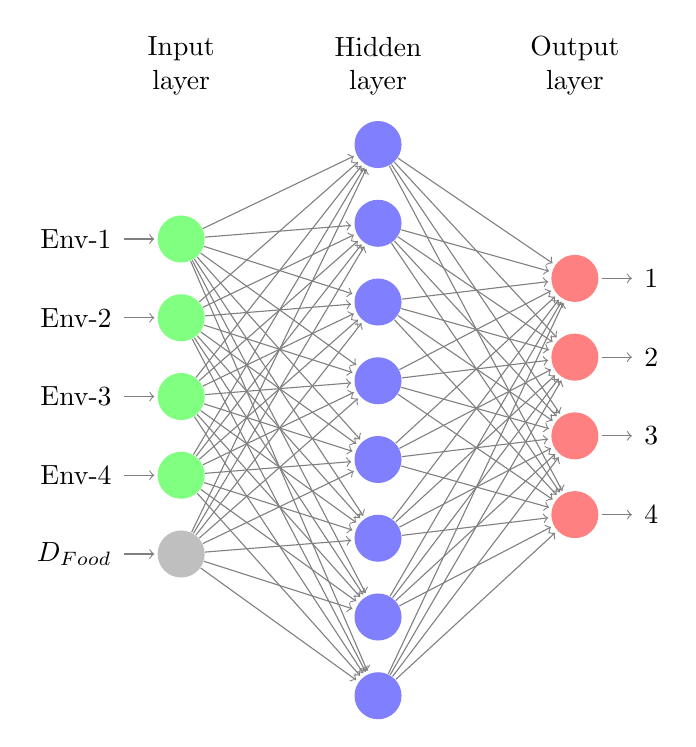
\begin{tikzpicture}[shorten >=1pt,->,draw=black!50, node distance=\layersep]
    \tikzstyle{every pin edge}=[<-,shorten <=1pt]
    \tikzstyle{neuron}=[circle,fill=black!25,minimum size=17pt,inner sep=0pt]
    \tikzstyle{input neuron}=[neuron, fill=green!50];
    \tikzstyle{output neuron}=[neuron, fill=red!50];
    \tikzstyle{hidden neuron}=[neuron, fill=blue!50];
    \tikzstyle{annot} = [text width=4em, text centered]

    \foreach \name / \y in {1,...,4}
        \node[input neuron, pin=left:Env-\y] (I-\name) at (0,-\y) {};

    \node[neuron, pin=left:$D_{Food}$](B-1) at (0,-5) {};
    
    \foreach \name / \y in {1,...,8}
        \path[yshift=1.2cm]
            node[hidden neuron] (H-\name) at (\layersep,-\y cm) {};

    \foreach \ind in {1,...,4}
    	\node[output neuron,pin={[pin edge={->}]right:\ind}, right of=H-\ind, yshift=-1.7cm] (O\ind) {};
    
    \foreach \source in {1,...,4}
        \foreach \dest in {1,...,8}
            \path (I-\source) edge (H-\dest);
	
    \foreach \dest in {1,...,8}
    	\path (B-1) edge (H-\dest);
        
    \foreach \source in {1,...,8}
    	\foreach \out in {1,...,4}
        	\path (H-\source) edge (O\out);

    % Annotate the layers
    \node[annot,above of=H-1, node distance=1cm] (hl) {Hidden layer};
    \node[annot,left of=hl] {Input layer};
    \node[annot,right of=hl] {Output layer};
\end{tikzpicture}
\caption{\label{fig:netstructure_evo}The network structure of the second evolutionary approach. The input layer consists of the four neighborhood around the head as well as a distance node to the food token.}
\end{center}
\end{figure}


%%%%%%%%%%%%%%%%%%%%%%%%%%%%%%%%%%%%%%%%%%%%%%%%%%%%%%%%%%%%%%%%%%%%%%
%%%%%%%%%%%%%%%%%%%%%%%%%%%%%%%%%%%%%%%%%%%%%%%%%%%%%%%%%%%%%%%%%%%%%%
\subsection{Q-Snake}
The Q-Snake implements a reinforcement learning approach. It is based on the idea of traditional Q-learning, where expected rewards, the Q-values, for every possible action in every possible state are represented in a tabular fashion. The Q-values in such a table are adjusted by reinforcement learning, in which the game is played repetitively and the rewards which are observed as a result of specific actions are propagated through the table.

In a game like snake a state depends not only on the positions of the (for the player controllable) snake head and food token, but also on the size of the snakes body and all its different orientations on the board. Therefor we end up with a state space for which a tabular representation is unfeasible.

At this point Deep Q-Learning Networks (DQN) come into play. Patented by \textit{Google Inc}, DQN describes the idea of encoding the Q-values in a neural network's weights and biases \cite{mnih2016}. This abstracts the in the tabular approach explicitly saved values into a non-linear approximation function. Originally scientists at Google presented this approach in the infamous so-called \textit{Atari paper} \cite{mnih2013}.

Similar to the first \textit{Evolved Snake} approach described above, the Q-Snake also receives the game board's state ($8x8$ matrix of integers ranging from 0 to 2) and rewards. In general the network receives a neutral reward while moving the snake around, a positive one when collecting a food token and a negative one when loosing (by crashing into the snake's body or the board's borders). 

Because the snake's body is of uniform color the network needs to receive information about the location of the head. In order to avoid hard coding this, the Q-Snake remembers the last state and the network itself receives a difference image of the current and the last board state.

\begin{figure}
  \centering
  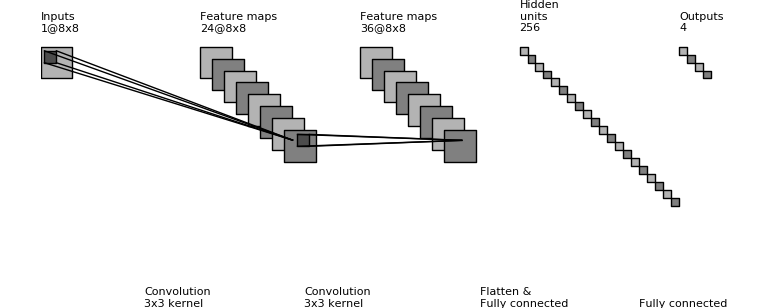
\includegraphics[width=\textwidth]{convnet_fig}
  \caption{\label{fig:q_snake_network}Q-Snake network structure.}
\end{figure}

\subsubsection{Network Structure}
In order to utilize the potential of local information the Q-Snake uses a convolutional neural network. In order to enable the network to learn non-linear mappings from states to actions and in accordance to previous works (e.g. \cite{mnih2013}), a multi layer network is used. Because of the rather small used board size and no observed improvement we opted for no-more than two convolutional and one fully connected hidden layers, as seen in Figure \ref{fig:q_snake_network}. All but the last layer use ReLu activation functions. For the output Q-values linear activations are used.

\subsubsection{Training}
During training the Q-Snake repeatedly plays the game and saves progress into a memory queue. The queue holds quadruples of $(state, action, reward, state')$, where $state'$ is the state which resulted from taking the specified action in the specified state. 

After the memory holds a certain amount of quadruples, the network starts training on mini-batches uniformly sampled from the memory. The minimal required memory size directly depends on the size of the mini-batches. While we, similar to the reference paper \cite{mnih2013}, make use of mini-batches of size 32, we also opted for a memory of 10 thousand instead of 1 million quadruples to reduce memory usage.

Training occurs on-line. After every action taken, the gradient descent back-propagation step is applied and the updated network decides on which action to take next from the updated state. In order to encourage exploration during training, the Q-Snake has a decaying probability to overrule the network's result and take a uniformly chosen random action instead. While initially this probability is $90\%$, it linearly decreases to a minimum $10\%$ after half of the scheduled training games.

While we played around with different rewards (e.g. higher positive reward to make the snake more aggressively hunt for food), in the end traditional +1/-1 rewards prove successful with enough training. Nevertheless, the initialization of weights and the learning rate and reward decay prove to be essential for the network's weights to not diverge.

\begin{figure}
    \centering
    \begin{subfigure}[b]{0.24\textwidth}
        
\includegraphics[width=\textwidth]{qsnake_snaps/1}
        \caption{Grow, grow}
    \end{subfigure}
    \begin{subfigure}[b]{0.24\textwidth}
        
\includegraphics[width=\textwidth]{qsnake_snaps/2}
        \caption{grow myself}
    \end{subfigure}
    \begin{subfigure}[b]{0.24\textwidth}
        
\includegraphics[width=\textwidth]{qsnake_snaps/3}
        \caption{gently on the direct}
    \end{subfigure}
    \begin{subfigure}[b]{0.24\textwidth}
        
\includegraphics[width=\textwidth]{qsnake_snaps/4}
        \caption{or indirect way}
    \end{subfigure}
    \begin{subfigure}[b]{0.24\textwidth}
        
\includegraphics[width=\textwidth]{qsnake_snaps/5}
        \caption{*nom nom*}
    \end{subfigure}
    \begin{subfigure}[b]{0.24\textwidth}
        
\includegraphics[width=\textwidth]{qsnake_snaps/6}
        \caption{I see this food}
    \end{subfigure}
    \begin{subfigure}[b]{0.24\textwidth}
        
\includegraphics[width=\textwidth]{qsnake_snaps/7}
        \caption{scenic route}
    \end{subfigure}
    \begin{subfigure}[b]{0.24\textwidth}
        
\includegraphics[width=\textwidth]{qsnake_snaps/8}
        \caption{life is good}
    \end{subfigure}
    \begin{subfigure}[b]{0.24\textwidth}
        
\includegraphics[width=\textwidth]{qsnake_snaps/9}
        \caption{*sizzle*}
    \end{subfigure}
    \begin{subfigure}[b]{0.24\textwidth}
        
\includegraphics[width=\textwidth]{qsnake_snaps/10}
        \caption{I'm a snake!}
    \end{subfigure}
    \begin{subfigure}[b]{0.24\textwidth}
        
\includegraphics[width=\textwidth]{qsnake_snaps/11}
        \caption{A predator}
    \end{subfigure}
    \begin{subfigure}[b]{0.24\textwidth}
        
\includegraphics[width=\textwidth]{qsnake_snaps/12}
        \caption{and cautious}
    \end{subfigure}
    \begin{subfigure}[b]{0.24\textwidth}
        
\includegraphics[width=\textwidth]{qsnake_snaps/13}
        \caption{Look at my tail!}
    \end{subfigure}
    \begin{subfigure}[b]{0.24\textwidth}
        
\includegraphics[width=\textwidth]{qsnake_snaps/14}
        \caption{A bit difficult to avoid}
    \end{subfigure}
    \begin{subfigure}[b]{0.24\textwidth}
        
\includegraphics[width=\textwidth]{qsnake_snaps/15}
        \caption{soo long..}
    \end{subfigure}
    \begin{subfigure}[b]{0.24\textwidth}
        
\includegraphics[width=\textwidth]{qsnake_snaps/16}
        \caption{Wait-what?! Ahh...}
    \end{subfigure}
    \caption{Example run of the Q-Snake}
    \label{fig:q_game}
\end{figure}

% \begin{figure}
%   \centering
%   \includemedia[width=0.6\linewidth,height=0.6\linewidth,activate=pageopen,passcontext,transparent,addresource=pysnake.mp4,flashvars={source=pysnake.mp4}]{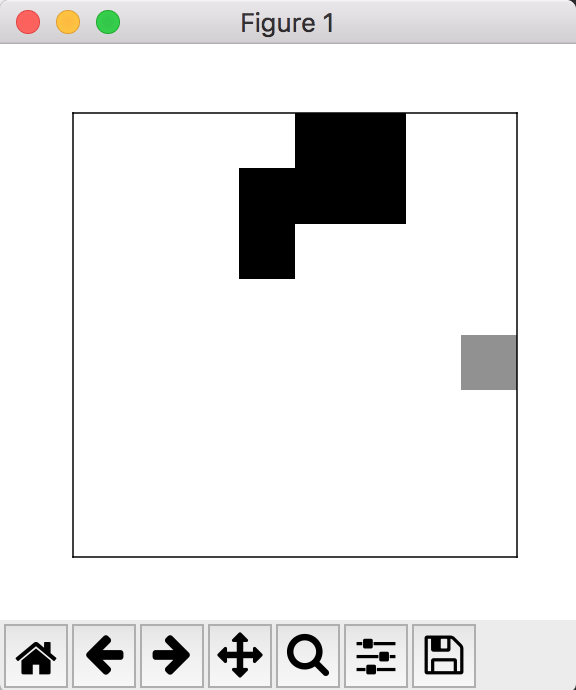
\includegraphics[width=0.6\linewidth]{SnakeBoard}}{VPlayer.swf}
%   \label{fig:q_snake_live}
%   \caption{Q-Snake playing a game after $55000$ games of training. Animated figure when viewed in modern PDF viewer.}
% \end{figure}


%%%%%%%%%%%%%%%%%%%%%%%%%%%%%%%%%%%%%%%%%%%%%%%%%%%%%%%%%%%%%%%%%%%%%%
%%%%%%%%%%%%%%%%%%%%%%%%%%%%%%%%%%%%%%%%%%%%%%%%%%%%%%%%%%%%%%%%%%%%%%
\subsection{Training Deep Neural Networks}
Training deep ANNs is expensive. In order to be able to train our networks and to test different structures of those networks we opted for GPU computing instances offered by Amazon Web Services. In order to save up to $80\%$ on the original on-demand prices we aggressively made use of so called \textit{spot instances}. Through these flexibly priced instances Amazon offers unused computing resources to the highest bidder. When bidding for such an instance one decides on a maximum price and then receives an instance if and keeps it as long as his maximum price is still higher than the current market price. Because an instance might be shut down at any time due to being outbid, one needs to be aware of potential data loss and should take measures (like regular backups) to prevent those.

Because prices are extremely fluctuating between different AWS regions and even within a region's different availability zones, we implemented a script which quickly determines the cheapest region, reserves an instance and prepares it for training neural networks using the official Tensorflow docker image. To easily manage multiple of those instances from a single local host machine we made use of the \textit{docker-machine} command line utility. Using this scheme we were able to train our implementations on otherwise not affordable Tesla K80 GPUs at an average price of approximately $0.14\$$US per hour.


%%%%%%%%%%%%%%%%%%%%%%%%%%%%%%%%%%%%%%%%%%%%%%%%%%%%%%%%%%%%%%%%%%%%%%
%%%%%%%%%%%%%%%%%%%%%%%%%%%%%%%%%%%%%%%%%%%%%%%%%%%%%%%%%%%%%%%%%%%%%%
\section{Performance Evaluation}
\label{sec:perf}
To evaluate the different strategies we first define three different metrics: the score, the number of steps, and the score-per-step ratio. The score $s$ is simply determined by the number of food items the snake eats during a game, or the final length $L$ minus the initial length $L_0$, in our case with $L_0 = 5$, this results in $s = L-5$. The number of steps is simply $N$ and counts the steps from the start to either win or loss. The score-per-step ratio is then simply the quotient of the score the number of steps: $r = \frac{s}{N} = \frac{L-L_0}{N}$. Because of the way scores are calculated, it is possible that $N$ becomes 0. To avoid this, we only analyze the results for data where the score is positive.

To make the comparisons possible we have to fix the parameters: For all tests the board size is $8 \times 8$ and the walls are enabled, that means it is not possible for the player to let the snake walk out of the boundaries and come back on the opposite side. Additionally the head is not colored with a special color but just the normal snake color.

For our baseline we let 6 people play the game four 
times each and record each of their step counts and scores. Additionally we  record 13790 runs of the systematic snake. The performance numbers of the networks stem from the saved weights available on myshare (see section~\ref{sec:res} for links to download them and the README on GitHub for ways to run the files). Those have been run with the reported number of steps to calculate the performance statistic.

In the end, we were not too happy with either the evolutionary nor the Q-learning approach. While at least Q-learning prove to be quite successful in initial phases of the game, it did not manage to actually win (fill the whole board) by any means.

\begin{table}
	\centering
    \small
	\begin{tabular}{l|r|r|r|r|r}
        Approach & Samples & Invalid & Min:Median:Max $N$ & Min:Median:Max $s$ & Min:Mean:Max $r$ \\\hline\hline
        Human & $24$ & $2$ & $18.00:310.00:814.00$ & $5.00:29.00:58.00$ & $0.05:0.11:0.28$ \\\hline
        Systematic & $13970$ & $0$ & $638.00:918.00:1213.00$ & $58.00:58.00:58.00$ & $0.05:0.06:0.09$  \\\hline
        Evolutionary & $30$ & $0$ & $1.00:9.00:\infty$ & $0.00:0.00:1.00$ & $0.00:0.00:0.06$ \\\hline
        Q-learning & $294$ & $0$ & $5.00:82.00:227.00$ &$1.00:8.00:18.00$ & $0.20:0.10:0.08$ \\\hline\hline
    \end{tabular}
	\caption{\label{tab:performance}The performance of different approaches.}
\end{table}


%%%%%%%%%%%%%%%%%%%%%%%%%%%%%%%%%%%%%%%%%%%%%%%%%%%%%%%%%%%%%%%%%%%%%%
%%%%%%%%%%%%%%%%%%%%%%%%%%%%%%%%%%%%%%%%%%%%%%%%%%%%%%%%%%%%%%%%%%%%%%
\section{Discussion}
Playing the Snake game is at first glance not a specifically hard or complex task. Yet it was quite challenging to train the neural networks to play the game. In the end the whole evolutionary approach did not sufficiently work and only the Q-Snake was able to perform reasonably good (although being outperformed by the systematic approach in the long run, see Section \ref{sec:perf}). During writing the code we learned how frustrating finding the error in a neural network is and how heavily such approaches rely on the availability of computational power. Although from the herein presented results a conclusion could be drawn that neural networks for this specific problem are not an optimal solution, we see potential for growth.

The Q-learning approach showed a lot of potential. A main problem here was the training required before it demonstrated reasonable playing performance. From what we saw this seems to be the case, because game states occurring later in the game are significantly different from earlier states, wherefore a deducting from rewards in earlier states to expected rewards in later states is hard. There are different enhancements which might help to tackle that specific problem. One for example is the introduction of a prioritized memory queue, where relevant states (those which are connected with positive and negative rewards) are more prominently trained on than reoccurring, more insignificant states. Additionally keeping a bigger memory queue might help to reduce the problem of forgetting already seen states.


%%%%%%%%%%%%%%%%%%%%%%%%%%%%%%%%%%%%%%%%%%%%%%%%%%%%%%%%%%%%%%%%%%%%%%
%%%%%%%%%%%%%%%%%%%%%%%%%%%%%%%%%%%%%%%%%%%%%%%%%%%%%%%%%%%%%%%%%%%%%%
\section*{Resources}\label{sec:res}
\begin{enumerate}
\item All source code is hosted on \href{https://github.com/ahoereth/pysnake}{GitHub}
\item Evolutionary network can be found \href{https://myshare.uni-osnabrueck.de/f/9c903b6994/?raw=1}{here}
\item Q-Snake network can be found \href{https://myshare.uni-osnabrueck.de/f/a893e165f0/?raw=1}{here}
\item Values of the human performance can be found \href{https://myshare.uni-osnabrueck.de/f/d24eb213af/?raw=1}{here}
\item Systematic performance can be found \href{https://myshare.uni-osnabrueck.de/f/b3a04d4ac6/?raw=1}{here}
\item Complete MyShare \href{https://myshare.uni-osnabrueck.de/d/a26302e43c/}{folder} 
\end{enumerate}

\bibliographystyle{alpha}
\bibliography{sample}

\end{document}
